\documentclass[a4paper,10pt]{article}
\usepackage[spanish]{babel}
\usepackage[latin1]{inputenc}
\usepackage{anysize} % Soporte para el comando \marginsize
\usepackage{listings}
\usepackage{formular}
\usepackage[pdftex]{graphicx}
\usepackage{setspace}
\usepackage{booktabs}



\DeclareGraphicsExtensions{.pdf,.png,.jpg}

\usepackage{color}
\definecolor{gray97}{gray}{.97}
\definecolor{gray75}{gray}{.75}
\definecolor{gray45}{gray}{.45}

\lstset{ frame=Ltb,
     framerule=0pt,
     aboveskip=0.5cm,
     framextopmargin=3pt,
     framexbottommargin=3pt,
     framexleftmargin=0.4cm,
     framesep=0pt,
     rulesep=.4pt,
     backgroundcolor=\color{gray97},
     rulesepcolor=\color{black},
     %
     stringstyle=\ttfamily,
     showstringspaces = false,
     basicstyle=\small\ttfamily,
     commentstyle=\color{gray45},
     keywordstyle=\bfseries,
     %
     numbers=left,
     numbersep=15pt,
     numberstyle=\tiny,
     numberfirstline = false,
     breaklines=true,
   }

% minimizar fragmentado de listados
\lstnewenvironment{listing}[1][]
   {\lstset{#1}\pagebreak[0]}{\pagebreak[0]}

\lstdefinestyle{consola}
   {basicstyle=\scriptsize\bf\ttfamily,
    backgroundcolor=\color{gray75},
   }

\lstdefinestyle{C}
   {language=C,
   }


\renewcommand*\lstlistingname{Listado}


\marginsize{3cm}{3cm}{2.5cm}{2.5cm}
\setlength{\parindent}{25pt}

%opening
\title{\textbf{ Wireless communications
in NS3}\\ Simulating wireless communications}
\author{Alejandro Juli\'an Ferro Bejerano}

\begin{document}


\maketitle

\begin{figure}[!h]
\centering
   
\includegraphics[width=8cm]{escudo_esi.jpg}
\end{figure}

\newpage

\tableofcontents

\newpage

\section{Objetives}

The main objective of this documents is to understand wireless communications and guide student in
its first simulation process through NS3 simulator.

\singlespacing
To do so, we will answer some fundamental questions. Let's look

\section{Changing the script}
Starting with the original example stats and responds as would the following activities.

\subsection{increment the distances used in each iteration of the simulation to: 25 50 75 100 125 145 147
150 152 155 157 160 162 165 167 170 172 175 177 180 185 190 195 200 210 220 230 240 250
300 350 400 450 500 600 750 1000}

\subsection{Reduce the number of iterations for each distance from five to one}

\subsection{Adjust the x-axis of the gnuplot script to show results of the new distance}

\begin{figure}[h]
        	\centering
    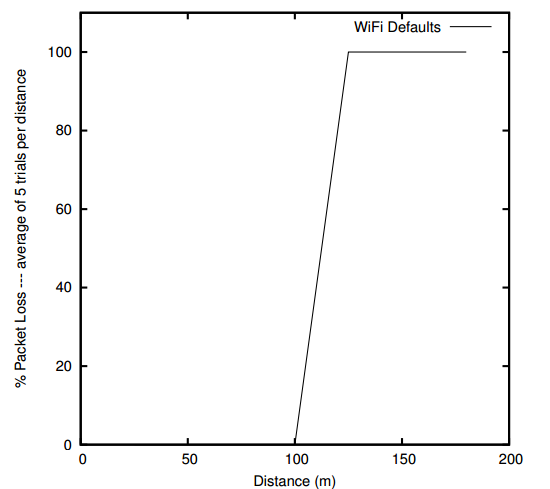
\includegraphics[scale=0.75]{basegraph.png}
    \caption{Graphic generated by example stats of NS3}
    \label{fig:inicio}
        \end{figure}


\section{Changing the antenna parameters of simulation}

\section{The loss model}

\subsection{Descripci\'on cualitativa}
Una breve definici\'on de la informaci\'on que nos pueden ofrecer los diferentes campos de la base de datos:
\begin{itemize}
\item \textbf{Date:} fecha en la que tiene lugar el accidente con el formato ``Month DD, YYYY''. Ejemplo: ``October 01, 1916 ''.
\item \textbf{Time:} hora local a la que ocurre el accidente en formato ``HH:MM''. Ejemplo: ``18:30''.
\item \textbf{Location:} lugar aproximado  donde tiene lugar el accidente.
\item \textbf{Summary:} descripci\'on del accidente y causa si se conoce.
\end{itemize}


\section{Hip\'otesis}
Se pretende clasificar cierto vuelo en una categor\'ia de riesgo definida previamente seg\'un su nivel de peligrosidad. Esto se har\'a en base a las caracter\'isticas del vuelo que es objeto de estudio.
\singlespacing
En la clasificaci\'on ser\'a necesario emplear un n\'umero impar de categor\'ias para que exista un elemento central sobre el que pivotar, comprendiendo en el presente caso cinco niveles de mayor a menor peligrosidad. Estas categor\'ias son:



\pagebreak
	Los par\'ametros que se tendr\'an en cuenta para definir esta medida de riesgo y poder realizar una posterior clasificaci\'on son: hora, origen, destino, escalas, la compa\~n\'ia a\'erea y modelo de avi\'on.
    \singlespacing
	Estas caracter\'isticas del vuelo han sido escogidas por ser las que con mayor precisi\'on especifican los aspectos que pueden afectar a la peligrosidad del vuelo.
    \singlespacing
	El sistema ser\'a de ``Segmentaci\'on'' ya que ante el valor de determinadas entradas (hora, origen, destino, escalas, la compa\~n\'ia a\'erea y modelo de avi\'on) este seleccionar\'a de entre distintas clases predefinidas la clase que m\'as se ajuste.



\singlespacing
\begin{table}[htbp]
\centering
\begin{tabular}{p{4cm} p{8cm}}
\hline \hline
Campos eliminados & Descripci\'on\\
\hline \hline
Registration & Es el registro de la ICAO, se ha decidido eliminarlo debido a que no es relevante para estimar el riesgo o peligrosidad de las rutas.\\
\hline
cn/ln & N\'umero de construcci\'on o n\'umero de serie / l\'inea o identificaci\'on del fuselaje. Se desprecier\'an los datos relativos al fuselaje ya que no es uno de los atributos determinantes de riesgo del vuelo.\\
\hline
Flight & El n\'umero de vuelo asignado por el operador de la aeronave, no es interesante ya que cada aerol\'inea tiene su propio sistema de numeraci\'on, es demasiado singular para tenerlo en cuenta.\\
\hline \hline

\end{tabular}
\caption{Campo ``Operator''.}
\label{tabla:autores}
\end{table}

    \singlespacing
	Como resultado de esta selecci\'on se obtiene una tarjeta de datos se obtiene una tarjeta de datos compuesta por vuelos que son comerciales y posteriores a 1950, sin los campos anteriormente mencionados.
    \singlespacing
	La tarjeta de datos resultante cubre razonablemente el espacio de entradas y salidas, ya que con ella manejamos datos como el modelo de avi\'on, operadora, ruta, fecha y hora de los accidentes ocasionados en vuelos comerciales relativamente actuales, y que son suficientes para determinar el nivel de peligrosidad de un vuelo.

\subsection{Preprocesamiento previo descriptivo}
Ante la incertidumbre de algunos factores se debe determinar la completitud de la base de datos, es decir, analizar la carencia, imprecisi\'on e incertidumbre y estimar el nivel de ruido de la base de datos para ver si es tolerable.
\singlespacing
	Se observan algunos registros con el valor ``?'' referentes al campo ``Time''. Se ha decidido tomar como valor por defecto la hora en la que m\'as sucesos tengan lugar del resto de registros de este campo en estos casos. Algunos registros del campo ``Time'' tienes adem\'as de la hora el par\'ametro c, que indica que la hora est\'a en formato Central European Time, y el par\'ametro Z, en este caso el formato estar\'a en Hora Zul\'u; se ha dise\~nado un algoritmo que busque los registros en los que se dan estos casos y se transformen a hora local.
    \singlespacing
	Se eliminan las entradas en las que el campo `AC Type'' es ``?'', ya que no se puede adivinar el modelo del avi\'on al que hace referencia el accidente. Posteriormente y por el mismo motivo tambi\'en se eliminan las entradas en las que el campo `Operator'' es ``?''.
    \singlespacing
	En algunos registros de distintos campos se han detectado errores l\'exicos que causar\'an problemas en el procesamiento posterior de los datos. La lista de errores detectados y la soluci\'on aplicada es la siguiente.

\singlespacing
\begin{table}[htbp]
\centering
\begin{tabular}{p{5cm} p{7cm}}
\hline \hline
Error& Soluci\'on \\
\hline \hline
Pico X, pico Y de Monte Kilimajaro &Monte Kilimajaro\\
\hline
Sept-+le& Sept-\^Iles\\
\hline
Sondrestr÷mfjord& Sondrestrom Fjord\\
\hline
S\'Oo Tom\'U& S\~ao Tom\'e\\
\hline
Reykjav\'Yk& Reykjav\'ik\\
\hline
Crici·ma& Crici\'uma\\
\hline
B¯r Mogre´n& Bir Moghrein\\
\hline
Feij& Feij\'o\\
\hline
Gharda´a& Gharda\"ia\\
\hline
Lbeck&  L\"ubeck\\
\hline
San Jernimo de Moravia& San Jer\'onimo de Moravia\\
\hline \hline
Otros& Se eliminan ``, X mile[s] of Y of Z'' \\
\hline
Otros& Se eliminan ``near '' y ``near of''. \\
\hline
Otros& Se eliminan ``X nm of Y of Z''\\
\hline \hline

\end{tabular}
\caption{Campos ``Location'' y ``Route''.}
\label{tabla:autores}
\end{table}

\begin{table}[htbp]
\centering
\begin{tabular}{p{2cm} p{10cm}}
\hline \hline
Se eliminan ``charter - '' y `` - charter''&\\
\hline
Se eliminan ``- air taxi'' y ``Air Taxi -''&\\
\hline \hline

\end{tabular}
\caption{Campo ``Operator''.}
\label{tabla:autores}
\end{table}

\pagebreak

\singlespacing
\begin{table}[htbp]
\centering
\begin{tabular}{p{3cm} p{7cm}}
\hline \hline
Campos eliminados& Descripci\'on\\
\hline \hline
Fatalities &Total de muertes a bordo, se sustituir\'a por dos nuevos campos, Fatalities\_Passengers y Fatalities\_Crew\\
\hline
Abordo&Total de personas a bordo,ser\'a sustituido por Aboard\_Passengers y Aboard\_Crew\\
\hline
Route & Indica la ruta completa o parcial antes de producirse el accidente, incluyendo las escalas. Se sustituir\'a por los campos Origen, Destino, y Escalas\\
\hline \hline
\end{tabular}
\caption{Campos eliminados.}
\label{tabla:autores}
\end{table}
\pagebreak
\begin{table}[htbp]
\centering
\begin{tabular}{p{5cm} p{5cm}}
\hline \hline
Campos introducidos &Descripci\'on\\
\hline \hline
\hline
Fatalities\_Passengers &N\'umero total de pasajeros fallecidos\\
\hline
Fatalities\_Crew&N\'umero total de tripulaci\'on fallecida\\
\hline
Aboard\_Passengers & N\'umero total de pasajeros a bordo\\
\hline
Aboard\_Crew &N\'umero otal de tripulaci\'on a bordo\\
\hline
Origen&El primer elemento del campo ``Route''\\
\hline
Destino& El \'ultimo elemento del campo ``Route''\\
\hline
Escalas & Los elementos intermedios entre Origen y Destino del campo ``Route'' o ´´ '' si no existe ninguno\\
\hline
Latitude/Longitud\_Location & Latitud  y longitud del lugar del accidente\\
\hline
Latitude/Longitude\_Origen&Latitud  y longitud del lugar del origen del vuelo\\
\hline
Latitude/Longitude\_Destino&Latitud  y longitud del lugar del destino del vuelo\\
\hline \hline
\end{tabular}
\caption{Campos eliminados.}
\label{tabla:autores}
\end{table}



\singlespacing
La funci\'on de similitud consta de cuatro subfunciones definidas espec\'ificamente para los atributos seleccionados. Estas son:

\begin{lstlisting}[style=C]

NodeContainer nodes;
nodes.Create (2);
NS_LOG_INFO ("Installing WiFi and Internet stack.");
WifiHelper wifi = WifiHelper::Default ();
NqosWifiMacHelper wifiMac = NqosWifiMacHelper::Default ();
wifiMac.SetType ("ns3::AdhocWifiMac");
YansWifiPhyHelper wifiPhy = YansWifiPhyHelper::Default ();
YansWifiChannelHelper wifiChannel = YansWifiChannelHelper::Default ();
wifiPhy.SetChannel (wifiChannel.Create ());
NetDeviceContainer nodeDevices = wifi.Install (wifiPhy, wifiMac, nodes);
\end{lstlisting}


\singlespacing
Por otro lado, los pesos asignados a los atributos para calcular la media quedaron de la siguiente manera:
\begin{itemize}
\item Los campos ``Pasajeros a bordo'', ``Tripulaci\'on a bordo'', ``Pasajeros fallecidos'', ``Tripulaci\'on fallecido'' y ``Fallecidos en tierra'' se mantuvieron con peso ``1''.

\item A ``Fecha'', ``Hora'', ``Escalas'' y ``Modelo'' se decidi\'o asignarles peso ``2''.

\item Finalmente, a ``Coordenadas lugar del accidente'', ``Coordenadas origen de la ruta'' y ``Coordenadas destino de la ruta'' se les asigna peso ``3''.

\end{itemize}
\pagebreak
\section{Futuros proyectos}
El principal objetivo es aplicar de forma m\'as precisa los algoritmos de text minining que sean de utilidad para obtener la informaci\'on del campo ``Summary'' que puede ser muy relevante a la hora de categorizar.
\singlespacing
Por otra parte se desarrollar\'a un sistema que consuma la informaci\'on a partir de los resultados obtenidos en el proyecto. La aplicaci\'on se encargar\'a de evaluar un vuelo previamente introducido y clasificarlo dentro de un nivel de peligrosidad seg\'un sus caracter\'isticas. La aplicaci\'on deber\'ia ser c\'omoda de usar por cualquier usuario medio, por tanto ser\'ia conveniente desarrollar una interfaz de usuario sencilla e intuitiva.
\singlespacing
Tambi\'en ser\'ia interesante cruzar la base de datos de accidentes con otra base de datos referente a sucesos climatol\'ogicos para poder ampliar el conocimiento sobre la causalidad de los accidentes y poder a\~nadir m\'as par\'ametros al an\'alisis de riesgo.

\section{Conclusi\'on}
 En la asignatura se pretende desarrollar un sistema completo basado en el proceso KDD, lo cual ha sido plasmado en el presente trabajo. Se han aplicado los conocimientos de teor\'ia pertenecientes a la asignatura, siguiendo el proceso estudiado en clase. Se han adquirido las competencias necesarias para obtener conocimiento a partir de grandes vol\'umenes de datos.
Se ha puesto de manifiesto que no se trata de un proceso trivial, ya que no se usa la  metodolog\'ia convencional. \singlespacing
Adem\'as existe la dificultad a\~nadida de la necesidad en algunos casos de utilizar conocimientos transversales a la hora de sintetizar los datos. Es necesario tambi\'en conocer el \'ambito del problema y las particularidades asociadas al mismo.

\section{Webgraf\'ia y herramientas}
\begin{itemize}
\item https://www.nsnam.org/doxygen/
\item \LaTeX
\end{itemize}



\end{document}
